\documentclass[12pt,openright,oneside,a4paper,english,french,spanish,brazil,sumario=tradicional]{abntex2}

% --- Inclusão de Pacotes ---
\usepackage[utf8]{inputenc}
\usepackage[T1]{fontenc}
\usepackage{graphicx}
\usepackage{amsmath}

% --- Formatação Rigorosa ABNT ---
\usepackage{times} % Fonte Times New Roman (usando times em vez de mathptmx para evitar bug interno do compilador)
\usepackage[alf]{abntex2cite} % Pacote ABNT para citações

% Força a fonte com serifa (Times) nos títulos de capítulos e seções
\renewcommand{\ABNTEXchapterfont}{\rmfamily\bfseries}
\renewcommand{\ABNTEXsectionfont}{\rmfamily\bfseries}
\renewcommand{\ABNTEXsubsectionfont}{\rmfamily\bfseries}
\renewcommand{\ABNTEXsubsubsectionfont}{\rmfamily\bfseries}

% Força o tamanho 12 (normalsize) para todos os títulos
\renewcommand{\ABNTEXchapterfontsize}{\normalsize}
\renewcommand{\ABNTEXsectionfontsize}{\normalsize}
\renewcommand{\ABNTEXsubsectionfontsize}{\normalsize}
\renewcommand{\ABNTEXsubsubsectionfontsize}{\normalsize}

% Pacote para garantir o recuo do primeiro parágrafo após os títulos (Regra ABNT)
\usepackage{indentfirst}

% Ajusta a distância entre o título do capítulo/seção e o texto para ficar com o espaço correto (1 linha)
\setlength{\afterchapskip}{\baselineskip}
\setaftersecskip{\baselineskip}
\setaftersubsecskip{\baselineskip}
\setaftersubsubsecskip{\baselineskip}

% Adicione outros pacotes necessários aqui


% --- Configurações da UEA (Autor, Título, etc.) ---
% --- Criação de Variáveis Customizadas ---
\providecommand{\imprimiravaliador}{}
\newcommand{\avaliador}[1]{\renewcommand{\imprimiravaliador}{#1}}

\autor{MATHEUS COSTA SOARES DE AZEVEDO}
\titulo{DESENVOLVIMENTO DE UMA SOLUÇÃO DE \textit{SOFTWARE} EM LINGUAGEM C PARA SUPORTE À IMPLEMENTAÇÃO DE \textit{ASSET ADMINISTRATION SHELL} EMBARCADOS APLICADOS À INDUSTRIA 4.0}
\orientador{Rubens de Andrade Fernandes, Dr.}
\avaliador{Bruno da Gama Monteiro, Me.}

\local{Manaus}
\data{2026}


\preambulo{Projeto de pesquisa desenvolvido durante a disciplina de Trabalho de Conclusão de Curso I e apresentado à banca avaliadora do curso de Engenharia Eletrônica da Escola Superior de Tecnologia da Universidade do Estado do Amazonas, como pré-requisito para obtenção do título de Engenheiro em Eletrônica.}

% --- Configurações de Formatação de Parágrafo ABNT ---
\setlength{\parindent}{1.5cm} % Recuo da primeira linha do parágrafo
\setlength{\parskip}{0.2cm}   % Espaço entre um parágrafo e outro
\OnehalfSpacing               % Espaçamento de 1.5 entre linhas

% --- Estilo de Página (Cabeçalhos) ---
% Força o estilo 'abntheadings' a ser 'simple', o que remove a linha e o nome do capítulo
% do topo da página, deixando apenas o número da página no canto superior direito.
\aliaspagestyle{abntheadings}{simple}

% --- Configurações de Links do PDF ---
% Isso remove as caixas vermelhas em volta dos itens do sumário e deixa tudo em texto preto normal
\hypersetup{
    colorlinks=true,
    linkcolor=black,
    citecolor=black,
    filecolor=black,
    urlcolor=black
}

% --- Traduções e Textos ---
\addto\captionsbrazil{
  \renewcommand{\contentsname}{SUMÁRIO}
  \renewcommand{\bibname}{REFERÊNCIAS}
  \renewcommand{\listfigurename}{LISTA DE ILUSTRAÇÕES}
}


\begin{document}

% --- Elementos Pré-Textuais ---
\pretextual
\begin{folhaderosto}
\thispagestyle{empty} % Remove qualquer cabeçalho ou número de página solto

% Autor no topo
\begin{center}
    {\ABNTEXchapterfont\bfseries\large\imprimirautor}
\end{center}

\vspace{5cm} % Espaçamento fixo entre Autor e Título

% Título centralizado
\begin{center}
    {\ABNTEXchapterfont\bfseries\large\imprimirtitulo}
\end{center}

\vspace{2.5cm} % Espaçamento entre Título e Preâmbulo

% Preâmbulo alinhado perfeitamente na metade direita da página
\begin{flushright}
    \begin{minipage}{0.5\textwidth}
        \SingleSpacing
        \imprimirpreambulo
    \end{minipage}
\end{flushright}

\vspace{2.5cm} % Espaçamento entre Preâmbulo e Assinatura

% Orientador e assinatura centralizados
\begin{center}
    Orientador: \imprimirorientador
    
    \vspace{1.2cm} % Espaço para a caneta
    
    \rule{8cm}{0.15mm}
\end{center}

\vspace*{\fill} % Empurra o bloco de data exatamente para o rodapé

% Local e Data
\begin{center}
    {\large\imprimirlocal}
    \par
    {\large\imprimirdata}
\end{center}

\end{folhaderosto}


\pdfbookmark[0]{\contentsname}{toc}
\tableofcontents*
\cleardoublepage

\chapter*{INTRODUÇÃO}
\addcontentsline{toc}{chapter}{INTRODUÇÃO}

A consolidação da Indústria 4.0 transformou fundamentalmente os paradigmas da manufatura moderna, promovendo a digitalização e a interconexão de sistemas cibernéticos e físicos no chão de fábrica \cite{kagermann2013}. Nesse cenário de constante evolução tecnológica, surge a necessidade de soluções capazes de representar digitalmente os ativos industriais de forma padronizada, interoperável e altamente reutilizável. Para suprir essa demanda semântica, o \textit{Asset Administration Shell} (AAS) foi estabelecido como o padrão central para a implementação de Gêmeos Digitais, permitindo agrupar todas as propriedades, parâmetros e documentações de um ativo sob uma estrutura unificada \cite{zhang2025, olaya2025}.

Apesar da comprovada relevância do modelo AAS para atingir a verdadeira interoperabilidade exigida pela arquitetura RAMI 4.0 \cite{plattform2016}, a sua adoção prática enfrenta barreiras estruturais significativas nas camadas inferiores da pirâmide de automação. As bibliotecas e implementações do AAS atualmente disponíveis no mercado e na academia são, em sua grande maioria, voltadas para ambientes computacionais de alto desempenho, que contam com farta disponibilidade de memória RAM, grande poder de processamento e robusta infraestrutura de sistemas operacionais tradicionais \cite{pribis2021}, desta forma, a adoção de AAS em larga escala é inviável. 

Diante desse contexto, o presente trabalho se propõe a investigar e desenvolver uma solução otimizada de um AAS embarcado. O objetivo é fornecer uma implementação nativa e eficiente de modo a viabilizar, na prática, a adoção do conceito de Gêmeos Digitais em larga escala. Para isso, o documento descreve a construção de uma biblioteca baseada na arquitetura ESP32 com o sistema operacional de tempo real \textit{FreeRTOS}, aliando as capacidades de instrumentação física aos protocolos de comunicação semântica, como o OPC UA \cite{opcfoundation2026}.
\clearpage

% --- Elementos Textuais ---
\textual
% Desativa a quebra de página automática entre capítulos e força uma quebra de parágrafo com espaço
\renewcommand{\clearforchapter}{\par\vspace{1.0cm}}
\setlength{\beforechapskip}{0pt}

\chapter{TEMA}
Desenvolvimento de uma solução de \textit{software} em linguagem C para suporte à implementação de \textit{asset administration shell} embarcados aplicados à indústria 4.0
\chapter{FORMULAÇÃO DO PROBLEMA}

Apesar da relevância da AAS, muitas implementações disponíveis são voltadas a
ambientes computacionais mais robustos, com maior disponibilidade de memória, proces-
samento e infraestrutura de software. Essa característica dificulta sua adoção em sistemas
embarcados de baixo custo, especialmente em microcontroladores utilizados em aplicações
distribuídas da Indústria 4.0, nos quais restrições de recursos computacionais são um fator
determinante de projeto.
\chapter{HIPOTÉSE}

% Seu texto começa aqui

\chapter{OBJETIVO}

\section{Objetivo Geral}

Desenvolver uma solução de \textit{software} nativa em linguagem C para a implementação de um AAS em sistemas embarcados, permitindo avaliar a sua eficiência, viabilidade e adequação operacional em dispositivos com restrição de recursos computacionais.

\section{Objetivos Específicos}

Para alcançar o objetivo geral, foram definidos os seguintes objetivos específicos:
\begin{alineas}
    \item mapear o estado da arte e as soluções de AAS para sistemas embarcados, identificando as abordagens atuais, bem como suas limitações e lacunas tecnológicas;
    \item estabelecer os requisitos funcionais e não funcionais da biblioteca proposta, orientando-se pelos modelos padronizados do AAS, pelas demandas do protocolo OPC UA e pelas restrições do microcontrolador;
    \item implementar as funcionalidades centrais da biblioteca proposta, integrando a estrutura do AAS às rotinas de aquisição de dados e comunicação de rede;
    \item desenvolver um protótipo físico focado na instrumentação de grandezas elétricas para servir como um ambiente de validação prático (AAS Tipo 2);
    \item avaliar o desempenho, a estabilidade e o consumo de recursos da solução implementada, atestando sua eficiência em relação a implementações herdadas de ambientes computacionais mais robustos.
\end{alineas}

\chapter{JUSTIFICATIVA}

O projeto apresentado se justifica porque as implementações atuais de AAS são, em sua maioria, pensadas para ambientes
computacionais mais robustos, o que dificulta e, em muitos casos, inviabiliza sua adoção em larga escala em sistemas
embarcados. Assim, o desenvolvimento de um SDK nativo em C busca oferecer aos programadores uma ferramenta
mais adequada para implementar AAS em microcontroladores, tornando esse processo mais viável, eficiente e acessível.

O projeto utilizará conhecimentos adquiridos durante o curso de Engenharia Eletrônica, principalmente das disciplinas:
Projetos de Sistemas Microprocessados, Sistemas Operacionais Embarcados, Automação Industrial e Testabilidade e Segurança de Software Embarcado.
\chapter{REFERENCIAL TEÓRICO}

\section{QUEIMADAS NA FLORESTA AMAZÔNICA}

\section{INTERNET OF THINGS}

\section{LORA}

\section{MICROCONTROLADOR ESP32}

\subsection{Módulo ESP32 LoRa da Heltec}

\section{SENSORES}

\section{SERVIDOR TTN}

\chapter{METODOLOGIA}

O trabalho em questão consistirá em uma pesquisa aplicada, com o objetivo de realizar um estudo exploratório fundamentado em material bibliográfico e ensaios de laboratório. Serão utilizados os procedimentos técnicos de pesquisa bibliográfica e experimental. O percurso metodológico adotará o método de abordagem hipotético-dedutivo, complementado pelo método de procedimento monográfico para a sua estruturação e elaboração. No que tange à coleta de dados referentes ao desempenho do microcontrolador, será feito o uso de documentação indireta. A análise e a interpretação desses dados ocorrerão primariamente de forma qualitativa e global, avaliando o comportamento sistêmico da solução.

Inicialmente, será realizada uma revisão sistemática de literatura abordando as áreas centrais que permeiam o projeto: arquiteturas de microcontroladores modernos, sensores e instrumentação, sistemas eletrônicos de tempo real, Sistemas Operacionais Embarcados e as diretrizes do AAS na Indústria 4.0.

Complementarmente à fundamentação teórica, será realizado o estudo das bibliotecas de \textit{software} necessárias para o desenvolvimento do projeto. No escopo da biblioteca que será desenvolvida, destacam-se a avaliação de pilhas compatíveis com o protocolo OPC UA, como a \textit{open62541}, bibliotecas eficientes para serialização e manipulação de arquivos JSON em C/C++, como a \textit{cJSON}, além dos componentes nativos e \textit{drivers} fornecidos pelo \textit{framework} ESP-IDF.

Em seguida, serão desenvolvidos os códigos-fonte da biblioteca proposta neste trabalho. A implementação será focada em arquitetar um núcleo leve capaz de hospedar o AAS dentro das restrições de memória do microcontrolador, integrando as rotinas de comunicação e armazenamento de dados de forma transparente. Adicionalmente, durante o ciclo de desenvolvimento, será realizada a elaboração dos testes unitários necessários para garantir a robustez das funções críticas do sistema, prevenindo falhas de alocação de memória e garantindo a correta serialização dos dados.

Para a validação prática do uso da biblioteca, será desenvolvido um Gêmeo Digital reativo, caracterizado como um AAS do Tipo 2. O planejamento desta fase iniciará com o levantamento das ferramentas e equipamentos de medição, englobando aparelhos como multímetro e osciloscópio para a verificação e calibração dos sinais elétricos.

O \textit{hardware} montado formará a plataforma física do componente, ilustrada na Figura \ref{fig:arquitetura_geral}, enquanto a biblioteca desenvolvida atuará no microcontrolador para disponibilizar os dados na rede.

\clearpage

\begin{figure}[htb]
    \centering
    \caption{Arquitetura geral proposta para a instrumentação do AAS}
    \label{fig:arquitetura_geral}
    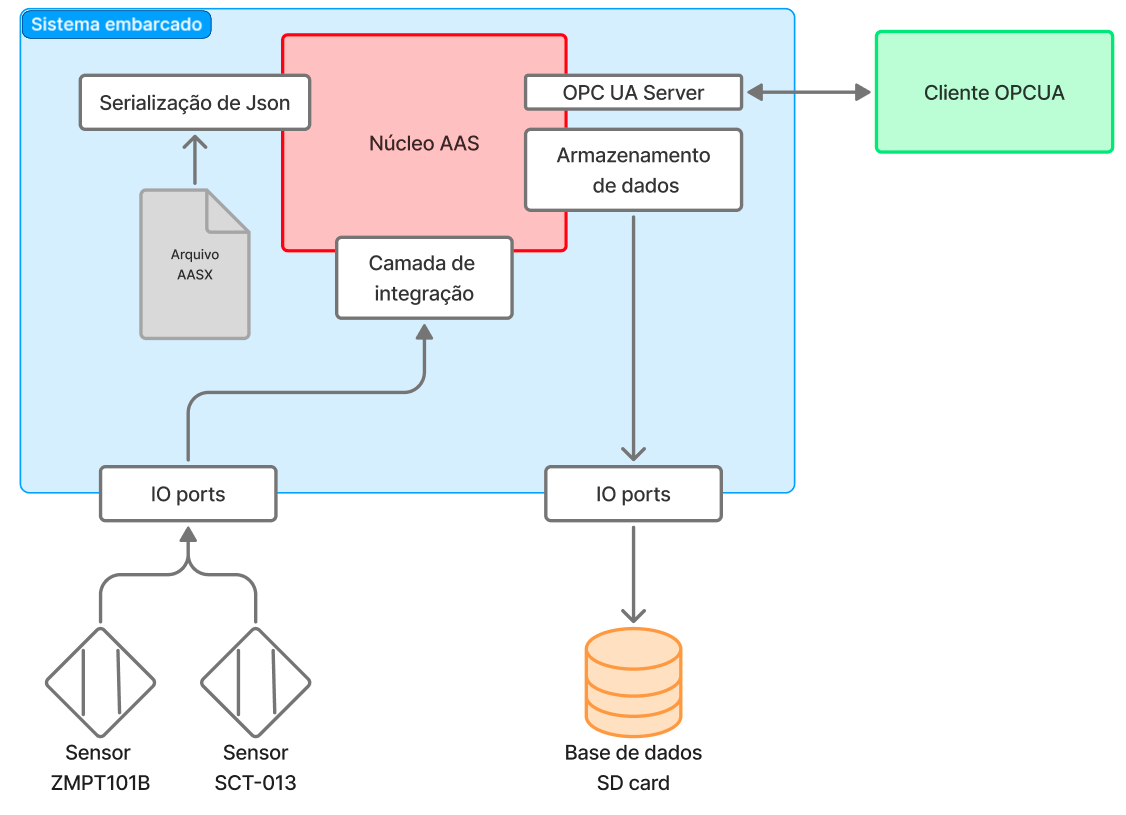
\includegraphics[width=0.60\textwidth]{figuras/arquitetura_geral.png}
    
    \fonte{Elaborado pelo autor.}
\end{figure}

A análise dos resultados será feita por verificação funcional da arquitetura. Serão observados o funcionamento da aquisição de dados, a continuidade da comunicação, a coerência dos registros armazenados e a atualização do gêmeo digital. Com isso, será possível medir e analisar o desempenho do microcontrolador como um AAS embarcado.

% --- Elementos Pós-Textuais ---
\postextual
\clearpage
\chapter{CRONOGRAMA}

\begin{figure}[htb]
    \centering
    \caption{Cronograma de execução do projeto}
    \label{fig:cronograma}
    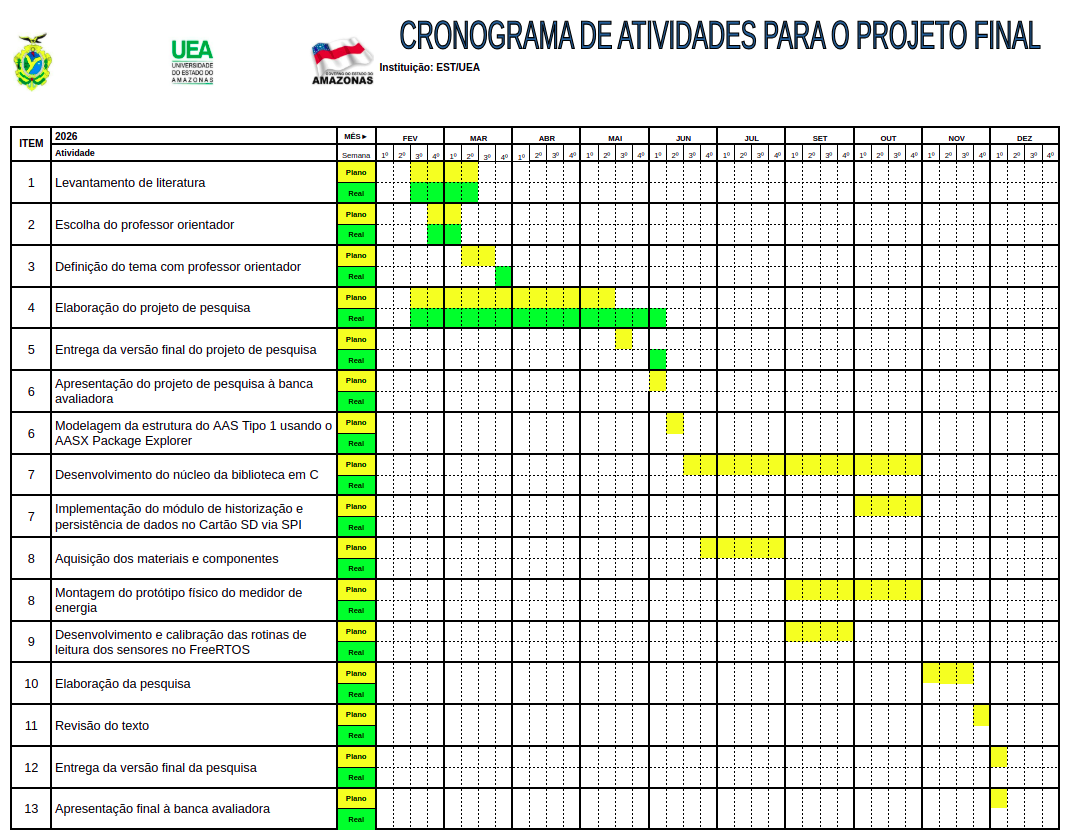
\includegraphics[width=1.0\textwidth]{figuras/cronograma.png}
    
    \fonte{Elaborado pelo autor.}
\end{figure}
\bibliographystyle{abntex2-alf}
\bibliography{referencias}
%\begin{folhadeaprovacao}
\thispagestyle{simple} % Para imprimir o número da página no topo como na imagem

\begin{center}
    \imprimirautor
    
    \vspace{2cm}
    
    \imprimirtitulo
\end{center}

\vspace{1.5cm}

\begin{flushright}
    \begin{minipage}{0.5\textwidth}
        \SingleSpacing
        \imprimirpreambulo
    \end{minipage}
\end{flushright}

\vspace{1.5cm}

\begin{center}
    Área de concentração: Sistemas Embarcados
    
    \vspace{0.8cm}
    
    Data da Apresentação: \underline{18 / 06 / 2026}.
    
    \vspace{0.4cm}
    
    Hora da Apresentação: \underline{18:30}.
    
    \vspace{1.2cm}
    
    PROTOCOLO DE ENTREGA DE PROJETO DE PESQUISA
    
    \vspace{0.4cm}
    
    BANCA EXAMINADORA
\end{center}

\begin{table}[htb]
\centering
{\renewcommand{\arraystretch}{1.6}
\begin{tabular}{|p{6cm}|c|>{\centering\arraybackslash}p{4cm}|}
\hline
\multicolumn{1}{|c|}{AVALIADOR} & DT RECEBIMENTO & RUBRICA \\ \hline
\imprimirorientador & \_\_\_\_/\_\_\_\_/\_\_\_\_ & \hspace{1cm} \\ \hline
\imprimiravaliador & \_\_\_\_/\_\_\_\_/\_\_\_\_ & \hspace{1cm} \\ \hline
\imprimirCoordenador & \_\_\_\_/\_\_\_\_/\_\_\_\_ & \hspace{1cm} \\ \hline
\end{tabular}
}
\end{table}

\vspace*{\fill}

\begin{center}
    \imprimirlocal
    \par
    \imprimirdata
\end{center}
\end{folhadeaprovacao}


\end{document}
